\section{Methods}\label{sec:Methods}

\subsection{Logistic Regression}
Logistic regression is a method of modeling the probability that a set of input variables $\bs{x}$ leads to an outcome or class $y_i$, $i = 1, 2, \dots K$, where $K$ is the number of possible classes. The model uses the logistic (or Sigmoid) function, which in the binary case with only two classes $y_i \in [0, 1]$, is given by
\begin{align}
    p(x) = \frac{e^x}{1 + e^x} = \frac{1}{1 + e^{-x}}
    \label{eq:sigmoid}
\end{align}
With instead a set of input variables $\bs{x}$, we can express the probabilities of each of the two outcomes as
\begin{align}
    p(y_i = 1 | x_i, \bs{\beta}) &= \frac{\exp(\bs{\beta}^Tx_i)}{1 + \exp(\bs{\beta}^Tx_i)}\\
    p(y_i = 0 | x_i, \bs{\beta}) &= 1 - p(y_i = 1 | x_i, \bs{\beta}),
\end{align}
where $\bs{\beta}$ are the coefficients which we want to estimate with our data.
Defining the set of all possible outcomes in our data set $\mathcal{D} = {(x_i, y_i)}$, and assuming that these samples are independent and identically distributed, the total likelihood for all possible outcomes in $\mathcal{D}$ can be approximated by the product of the individual probabilities\cite{hastie}[p.120] of a specific outcome $y_i$:
\begin{align}
    P(\mathcal{D}|\bs{\beta}) = \prod_{i=1}^{n} \left[ p(y_i= 1 | x_i, \bs{\beta} \right]^{y_i} \left[ 1 - p(y_i= 1 | x_i, \bs{\beta}) \right]^{1 - y_i}
\end{align}
Since in our model we aim to maximize the probability of seeing the observed data, we use the Maximum Likelihood Estimation principle, which by taking the log of the above equation leads to the log-likelihood function in $\bs{\beta}$:
\begin{align}
    \log P(\mathcal{D}|\bs{\beta}) = \sum_{i=1}^n \left[ y_i \log p(y_i = 1| x_i, \bs{\beta}) + (1 - y_i)\log(1 - p(y_i = 1 | x_i, \bs{\beta}))
    \right]
\end{align}
By taking the negative of the above expression and re ordering the logarithms, we arrive at what is known as the cross entropy:
\begin{align}
    \mathcal{C}(\bs{\beta}) = - \sum_{i=1}^n \left[ y_i\bs{\beta}^Tx_i - \log(1 + \exp(\bs{\beta}^Tx_i)) \right],
\end{align}
which we use as our cost function for logistic regression. Minimizing the cross entropy is the same as maximizing the log-likelihood:
\begin{align}
    \pdv{\mathcal{C}(\bs{\beta})}{\beta} = - \sum_{i=1}^n x_i(y_i - p(y_i=1 | x_i, \bs{\beta})) = 0,
    \label{eq:d_cross_entropy}
\end{align}
and computing the second derivative of this quantity gives
\begin{align}
    \pdv{\mathcal{C}(\bs{\beta})}{\bs{\beta}}{\bs{\beta}^T} = \sum_{i=1}^n x_ix_i^T p(y_i = 1 | x_i, \bs{\beta})(1 - p(y_i = 1 | x_i, \bs{\beta})).
\end{align}
Defining the diagonal matrix $\bs{W}$ with elements $p(y_i = 1 | x_i, \bs{\beta})(1 - p(y_i = 1 | x_i, \bs{\beta})$, $\bs{X}$ as the design matrix containing the data, $\bs{y}$ as the vector with our $y_i$ values and finally $\bs{p}$ as the vector of fitted probabilities, we can express the first and second derivatives in matrix form: 
\begin{align}
    \label{eq:cross_entropy_jacobian_hessian}
    \pdv{\mathcal{C}(\bs{\beta})}{\beta} &= -\bs{X}^T(\bs{y} - \bs{p})\\
    \pdv{\mathcal{C}(\bs{\beta})}{\bs{\beta}}{\bs{\beta}^T} &= \bs{X}^T\bs{WX},
\end{align}
also known as the Jacobian and Hessian matrices. The section below \ref{sec:gradient_descent} explains how we in practice solve this equation for $\bs{\beta}$ to obtain the optimal parameters of the predictors in the data set.

\subsection{Gradient Descent}\label{sec:gradient_descent}
A popular iterative method to finding the roots of an equation is the \textit{Newton-Ranphson method}\cite{Faul}[p. 116], which is derived from Taylor expanding a function $f$ in $x$ sufficiently close to the solution $x_0$. In the one-dimensional case it is expressed as 
\begin{align}
    x_{n+1} = x_n - \frac{f(x_n)}{f'(x_n)}.
\end{align}
In logistic regression, the function $f$ is substituted with the minimized expression for the cross entropy (eq. \ref{eq:d_cross_entropy}). We then have that the values $\bs{\beta}$ which maximize the log-likelihood can be found iteratively by
\begin{align}
\label{eq:newtons_method}
    \bs{\beta}^{n+1} &= \bs{\beta}^n - \left(\pdv{\mathcal{C}(\bs{\beta})}{\bs{\beta}}{\bs{\beta}^T}\right)^{-1}\left(\pdv{\mathcal{C}(\bs{\beta})}{\bs{\beta}}\right)\\
    &= \bs{\beta}^n - \left( \bs{X}^T\bs{WX} \right)^{-1} \left( -\bs{X}^T(\bs{y} - \bs{p}) \right),
\end{align}
where we have inserted the expressions for the Jacobian and Hessian matrices of the cross entropy (eq. \ref{eq:cross_entropy_jacobian_hessian}).

In optimization problems where computing the inverse of a matrix is impossible or simply too computationally demaning, using the Newton-Raphson method as is, is not a viable option. Looking back at the expression in equation \ref{eq:newtons_method}, one approach is to simply replace the inverse Hessian with a parameter $\eta$, referred to as the \textit{learning rate}. This leads to the method of \textit{steepest descent}\cite{Faul}[p. 52], which is based on the observation that if a function $F(\bs{x})$ is differentiable in the neighbourhood of a point $\bs{a}$, the function decreases the fastest in the direction of the negative gratient $-\nabla F(\bs{a})$. It then follows that the iterative method for finding the optimal $\bs{\beta}$ values in the logistic regression case, can be expressed as
\begin{align}
\label{gradient_descent}
    \bs{\beta}_{n+1} = \bs{\beta}^n - \eta \nabla\mathcal{C}(\bs{\beta}) = \bs{\beta}^n - \eta \left( \bs{X}^T(\bs{p} - \bs{y}) \right)
\end{align}
For a convex function and a small enough value for $\eta$, it is obvious that this method always converges to the global minimum, but its limitation is that it is sensitive to the initial conditions of $\bs{\beta}$ and may therefore get stuck in a local minima when dealing with a multivaried non-convex function. To avoid the shortcomings of the gradient descent method, we introduce an element of stochasticity in the way we calculate the gradients $\nabla \mathcal{C}(\bs{\beta})$. Instead of calculating the gradients on our whole data set $\bs{X}$, we randomly spilt the data into $M$ minibatches, and calculate the gradient for each minibatch. Denoting each minibatch as $B_k$ where $k=1, 2, ..., n/M$, the new approximation to the gradient is
\begin{align}
    \nabla \mathcal{C}(\bs{\beta}) = \sum_{i\in B_k}^{n/M} \nabla c_i(\bs{x_i}, \bs{\beta}),
\end{align}
where $k$ is chosen randomly with equal probability $[1, n/M]$.



\subsection{Neural Networks}


\emph{Artificial neural networks} (ANN) is a machine learning technique
inspired by the networks of neurons that make up the biological brain.
There are several different types of neural networks, and in this
project we use a multi-layer perceptron (MLP), where there is one or
more \emph{hidden layers} between the input and output layers, and each
hidden layer consists of several \emph{neurons}/\emph{nodes}. The signal will only go
in one direction, from the input layer to the output layer, which makes
this a \emph{feedforward neural network} (FNN). Additionally, all
nodes of a layer will be connected to every node on the previous
layer, which makes it a \emph{fully connected layer}. In this section we
will review the essential parts of how a neural network functions.


\subsubsection{Feed-forward}\label{feed-forward}

The basic idea of this kind of network is that the input information (i.
e. the features/predictors of our data set) \(y\), are passed through
all of the nodes in the hidden layers, until it ends up in the output
layer. Figure \ref{fig:nn} shows an example with three inputs, two hidden
layers with four nodes each, and one output. This process is called
\emph{forward feeding} of the network. Each input is multiplied by a
weight \(w_i\) when passed into a node, and the result is called
\(z_i\). The signal is then evaluated by an activation function
\(a(z_i) = a_i\), which then becomes the output from each node. Since
we are dealing with several observations, we assemble the weights
\(w_i\) into a matrix \(W\). Usually we add a bias \(b_i\) to each of the
nodes in a hidden layer, to prevent outputs of only zeros. The output
\(a_l\) of a layer \(l\) then becomes (where \(a_{l-1}\) is the output
from the previous layer):

\begin{align}
a_l = a(a_{l-1} W_l + b_l)
\label{eq:feedforward}
\end{align}

In the case of the first hidden layer, the input matrix \(X\), which contains the features of our data set, will take
the place of \(a_{l-1}\). The weights are usually initialized with
random values, for example using a normal or uniform distribution,
because if all the weights were the same, all nodes would give the
same output. In this project we use a standard normal distribution when
doing classification, but in the case for regression we use an
initialization proposed by Xavier Glorot and Yoshua
Bengio\cite{glorot}, where we scale the randomly
distributed weights by a factor \(1/\sqrt{n_{l-1} + n_l}\) (where \(n_{l-1}\) is
the size of the previous layer, and \(n_l\) is the size of the current
layer). The biases are given a small non-zero value, in our case
\(b_i = 0.01\) for all layers, in order to ensure activation.

\begin{figure}
\hypertarget{fig:nn}{%
\centering
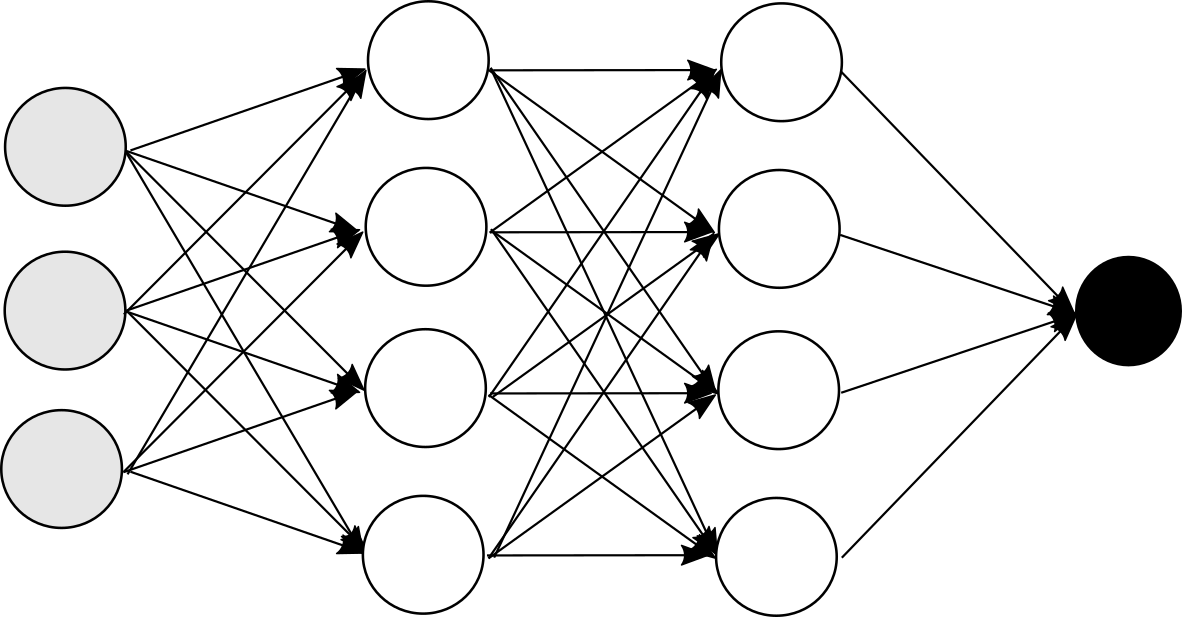
\includegraphics[scale=0.6]{Figures/Theory/neural-network.png}
\caption{Schematic neural network. The circles represent nodes, and
the colors indicate what layer they are a part of: Grey means input
layer, white means hidden layer and black means output layer. The arrows
show that all nodes of one layer is connected to each of the nodes
in the next layer; i. e. we have only fully connected
layers.}\label{fig:nn}
}
\end{figure}

\subsubsection{Activation functions}\label{activation-functions}

The choice of activation function may have a huge effect on the model,
and there are several options that may work depending on what data set
we want to process, how it is scaled and if it is a regression or
classification case. In a feed-forward neural network, we must have
activation functions that are non-constant, bounded,
monotonically-increasing and continous for the network to function
correctly on complex data sets. It is possible to choose different
activation functions for each hidden layer, but in this project we have
the same activation function throughout the networks we use.

Common choices for activation functions are the logistic/sigmoid
function, the Rectified Linear Unit function (ReLU) and the
\(\tanh\)-function\cite{geron}[p. 288]. For classification problems, the sigmoid function,
presented in equation \ref{eq:sigmoid}, is often preferred. This function
gives only output that is between \(0\) and \(1\), which is good when we
want to predict the probability as output of the network. In multiclass
classification problems the so-called softmax function is a better
choice, because it forces the sum of probabilites for the possible
classes to be 1, but for binary classification problems, like we have in
this project, the sigmoid function is sufficient.

For regression we use another common activation function, the ReLU
function:

\begin{equation}
\text{ReLU} = \begin{cases}
    0 & \text{if} \hspace{0.2cm} x < 0 \\
    x & \text{if} \hspace{0.2cm} x \geq 0
\end{cases}    
\end{equation}


\hypertarget{output-layer-and-back-propagation}{%
\subsubsection{Output layer and back
propagation}\label{output-layer-and-back-propagation}}

After the feed-forward process is done, the output layer will contain
the predictions of the neural network, which we will compare with the
true targets of our training data set. Based in this comparison, we will
adjust the weights and biases of the network in order to improve the
performance. Since the weights and biases usually are initialized
randomly, the first feed-forward iteration will most likely give very
wrong results. One feedforward pass is usually called an \emph{epoch},
and we choose the number of epochs based on how much ``training'' the
network needs in order to give satisfactory results. The process of
adjusting the weights and biases is called \emph{back propagation}.

The comparison between the output from the network \(\hat{y}\) and the
true targets of our training data set \(y\) is done with a predefined
cost function \(\mathcal{C}\). We want to minimize the cost, and to do
this we need to know how the weights and biases must be adjusted to
obtain a better result. This is done by calculating the gradient of the
cost function, and the exact derivation depends on how the cost function
is defined. Based on the derivative of the chosen cost function, and by using the chain rule\cite{hastie}[p. 396], one can show that in general terms the expression for the output error \(\delta_L\) becomes

\begin{equation}
    \label{eq:outputerror_general}
    \delta_L = \frac{\partial \mathcal{C}}{\partial a_L} \frac{\partial
a_L}{\partial {z_L}},
\end{equation}

and the back propagate error for the other layers $l = L-1, L-2, ..., 2$ is

\begin{equation}
    \delta_l = \delta_{l+1} W_{l+1}^T a'(z_l),
\end{equation}


where \(a'\) is the derivative of the activation function. The update of
the weights and biases for a general layer \(l\) is calculated by

\begin{align}
    W_l \leftarrow &= W_l - \eta a_{l-1}^T \delta_l,\\
    b_l \leftarrow &= b_l - \eta \delta_l,
\end{align}


where \(\eta\) is the learning rate, which specifies how much the
weights and biases should be adjusted for each back propagation. After the update of the weights and biases, we start a new epoch with another forward-feed of the network. We utilize minibatches, as described in the section above for gradient descent, in order to reduce the computational cost of the algorithm. The learning rate which is passed into the method is divided by the chosen batch size, to account for differences in the data size that is passed through each iteration.

In our classification problem, we use the binary cross-entropy as a cost
function:

\begin{equation}
\mathcal{C}_{\text{classification}} = - (y \log (p) + (1-y) \log (1 - p)),
\end{equation}

where \(p\) is the predicted probability of an observation, and \(y\) is
the true target, which will be either \(0\) or \(1\) since we have a
binary classification problem. The probabilities \(p\) is the same as
the output for our network \(\hat{y}\). Combining this with the sigmoid
as the activation function in the last layer, we use equation \ref{eq:outputerror_general} to get the formula for the output error:

\begin{equation}
    \label{eq:outputerror}
    \delta_L = \hat{y} - y.
\end{equation}

For regression we use a slightly modified version of the mean squared
error:

\begin{equation}
\mathcal{C}_{\text{regression}} = \frac{1}{2} \sum_{i=1}^n (\hat{y}_i - y_i)^2.
\end{equation}

The factor \(\frac{1}{2}\) is used to simplify the derivative of the
cost function, because if we use the identity function (which returns
the same values that is the input to the function, i. e. we have no activation function) as an activation
function in the last layer, the output error is the same as in equation
\ref{eq:outputerror}. This is very convenient, because we can use the same
calculation at the beginning of each back propagation whether we are doing classification or regression. A common
practice when using neural networks on regression problems is to use the
ReLU as activation function in the hidden layers, and then use the
identity function in the last layer\cite{geron}[p. 290].



\subsection{Error Metrics}

For classification, we use the accuracy score to measure how well our models perform, which is formulated as
\begin{align}
    \text{accuracy} = \frac{1}{n}\sum_{i=0}^n I(t_i = y_i).
\end{align}
where $t_i$ represents the target output, $y_i$ represents the output from our model, and $I$ is the indicator function, which returns $1$ if $y_i = t_i$ and $0$ otherwise.

We also make use of the so-called \textit{confusion matrix}, which is another commonly used error metric in classification problems. Instead of measuring only in how many instances the model has made a correct prediction over all, it gives the accuracy score of the model within each target class. For a two-class problem, the first row of the comfusion matrix will contain the values of the \textit{true negatives} and \textit{false negatives}, and the second row will show the values of \textit{false positives} and \textit{true positives}.

Finally, we use the area ratio in the \textit{cumulative gains chart} as a way of comparing the performance of our models. Such a chart has three curves which respectively represent the performance of a perfect classifier, a random classifier (baseline) and our model, with the horizontal axis representing the percentage of total data and the vertical axis representing the cumulative percentage of target data. The area ratio is defined as
\begin{align}
    \text{area ratio}=\frac{A_{model} - A_{baseline}}{A_{perfect} - A_{baseline}},
\end{align}
where a high area ratio would represent a good model.


\subsection{Description of the data}
For the classification case, we use a data set of credit card holders from a bank in Taiwan in 2005, which is available on the UCI website\footnote{UCI website: \href{https://archive.ics.uci.edu/ml/datasets/default+of+credit+card+clients}{https://archive.ics.uci.edu/ml/datasets/default+of+credit+card+clients}}. The original data set contains $30.000$ observations of whether the credit card holders default on their payment or not, and uses $23$ explanatory variables as the predictors for this binary outcome, where in total $22\%$ of the target variables are observations of defaults. 

We have chosen a couple of different avenues when it comes to preprocessing the data set, and in each case trained our models on it. The categorical features in the data set are those which specify gender, education and marital status, as well as payment status of previous months, with the remaining features being continuous. As explained on the UCI website, the history of previous payments are categorized from $-1$ to $9$, with $-1$ representing that the credit card holder has payed duly, and $1-9$ representing the number of months delay of payment. Because this feature has been categorized in this way, we have chosen to treat it as a categorical feature in one case, and as a continuous feature in another, to see which way of treating it gives the most accurate model. Categorical features have in both cases been one hot encoded, and continuous features have been min-max scaled to the range $[-1, 1]$. In our preprocessing of the data we have found some outliers in the explanatory variables which specify gender, education and marital status, and have opted to simply delete these entries. 
Since the data set we are operating on contains many more observations of non-defaults than defaults, we have also tried training our models on data in which we have randomly removed non-default entries from the training data, such that the default/non-default ratio is $1$:$1$ on the training data. 
In the case where the data was balanced, we have (prior to balancing) split it randomly into training data and test data, with $10\%$ being test data, and in the case of not balancing, $20\%$ was used for testing.

For the regression case we used the Franke function\cite{franke} to generate a data set. We used a grid size of $20\times20$ and a random generated noise with standard deviation $0.2$, and compared this to the results from our previous project\cite{project1}. Because of an unnoticed bug, the noise in the Franke function is only generated randomly along one axis, which means that the meshgrid gets the same noise value along one of the axes. This  results in a surface with smooth ridges, as we can see in figure \ref{fig:franke20}. The original plan was to have random noise along both axes in the meshgrid, but the bug was noticed too late in the analysis. This should however have little effect on the analysis of the machine learning methods, since the data was generated in the same way in our previous project, which is what we compare our results with.

\subsection{Benchmarks}
For logistic regression, we have constructed a test case where we compare the performance of our own implementation with Scikit Learn's \textit{LogisticRegressionCV} function on Scikit's breast cancer data set, by calculating the accuracy in both cases. The average difference in accuracy is in the order of $\epsilon = 10^{-4}$. In the case of classification with neural networks, we tested our code against Scikit Learn's \textit{MLPClassifier}, using the same breast cancer data set. Our code gave on average a better classification accuracy and a better area ratio compared to the results from Scikit Learn, and the difference was in the order of $10^{-1}$.

We also constructed a test case for regression, using the Franke data set with a $100 \times 100$ grid and a noise of $0.1$, where we benchmarked our neural network code against Scikit Learn's \textit{MLPRegressor}. With identical parameters passed into both our own code and the Scikit Learn's method, we obtained a difference in MSE and $R^2$ score in the order of $10^{-2}$.


\subsection{Source code}

The source code of this project is written in Python, and can be found in the GitHub repository at \url{https://github.com/ejhusom/FYS-STK4155/tree/master/project2/}. The repository contains our source code in the folder \texttt{src}, which consists of the following files:

\begin{itemize}
    \item \texttt{breastcancer.py}: Preprocessing of the breast cancer data
    \item \texttt{creditcard.py}: Preprocessing of the credit card data.
    \item \texttt{franke.py}: Preprocessing of the Franke data.
    \item \texttt{logistic\_classification.py}: Functions for analyzing the
        logisitic classification.
    \item \texttt{main.py}: Main entry to running the analysis.
    \item \texttt{nn\_classification.py}: Functions for analyzing the neural network when applied to classification problems.
    \item \texttt{nn\_regression.py}: Functions for analyzing the neural network when applied to regression problems.
    \item \texttt{pylearn}: Module containing our code for various machine learning methods, including logistic regression and neural networks.
\end{itemize}


